\documentclass[sigconf]{acmart}



\usepackage{booktabs} % For formal tables
\usepackage{wrapfig}
\usepackage{dblfloatfix}
\usepackage{hyperref}
\usepackage{balance}
\usepackage{colortbl}
\usepackage{mathtools}
\usepackage{cleveref}
\usepackage[shortlabels]{enumitem}
\usepackage[most]{tcolorbox}

\usepackage{picture}
\newcommand{\quart}[4]{\begin{picture}(100,6)%1
{\color{black}\put(#3,3){\circle*{4}}\put(#1,3){\line(1,0){#2}}}\end{picture}}
\newcommand{\quartr}[4]{\begin{picture}(100,6)%1
{\color{black}\put(#3,3){\color{red}\circle*{6}}\put(#1,3){\line(1,0){#2}}}\end{picture}}

\usepackage{pifont}% http://ctan.org/pkg/pifont

\newcommand{\cmark}{\ding{51}}%
\newcommand{\xmark}{\ding{55}}%

\newcommand{\bi}{\begin{itemize}[leftmargin=0.4cm]}
	\newcommand{\ei}{\end{itemize}}
\newcommand{\be}{\begin{enumerate}}
	\newcommand{\ee}{\end{enumerate}}


\makeatletter
\let\th@plain\relax
\makeatother

\definecolor{lightgray}{gray}{0.8}
\definecolor{darkgray}{gray}{0.6}
\definecolor{Gray}{gray}{0.85}
\definecolor{Blue}{RGB}{0,29,193}
\usepackage{tikz}
\usepackage{framed}
\usepackage[framed]{ntheorem}
\usetikzlibrary{shadows}

\theoremclass{Lesson}
\theoremstyle{break}

% inner sep=10pt,
\tikzstyle{thmbox} = [rectangle, rounded corners, draw=black,
fill=Gray!40]
\newcommand\thmbox[1]{%
	\noindent\begin{tikzpicture}%
	\node [thmbox] (box){%
		\begin{minipage}{.94\textwidth}%
		\vspace{-0.1cm}#1\vspace{-0.1cm}%
		\end{minipage}%
	};%
	\end{tikzpicture}}

\let\theoremframecommand\thmbox
\newshadedtheorem{lesson}{Result}

\newcommand{\tion}[1]{{Section }\ref{sect:#1}}

\usepackage{listings}
\definecolor{MyDarkBlue}{rgb}{0,0.08,0.45} 
\lstset{
    language=Python,
    basicstyle=\sffamily\fontsize{2.5mm}{0.7em}\selectfont,
    breaklines=true,
    prebreak=\raisebox{0ex}[0ex][0ex]{\ensuremath{\hookleftarrow}},
    frame=l,
    keepspaces=false,
    showtabs=false,
    columns=fullflexible,
    showspaces=false,
    showstringspaces=false,
    keywordstyle=\bfseries\sffamily,
    emph={ m, r, k, frontier, cf, f, g, n, tData, nrefs, cMax, inertia, gaps,trainData, testData, Word2Vec_model, trainX, trainY, cluster, svm_models, totalDlusterY, totalPredicted}, emphstyle=\bfseries\color{blue!50!black},
    stringstyle=\color{green!50!black},
    commentstyle=\color{red!50!black}\it,
    numbers=left,
    captionpos=t,
    escapeinside={\%*}{*)}
}

% Copyright
%\setcopyright{none}
%\setcopyright{acmcopyright}
%\setcopyright{acmlicensed}
\setcopyright{rightsretained}
%\setcopyright{usgov}
%\setcopyright{usgovmixed}
%\setcopyright{cagov}
%\setcopyright{cagovmixed}


% DOI
\acmDOI{10.475/123_4}

% ISBN
\acmISBN{123-4567-24-567/08/06}

%Conference
\acmConference[WOODSTOCK'97]{ACM Woodstock conference}{July 1997}{El
  Paso, Texas USA} 
\acmYear{1997}
\copyrightyear{2016}


\acmArticle{4}
\acmPrice{15.00}

% These commands are optional
%\acmBooktitle{Transactions of the ACM Woodstock conference} 


\begin{document}
\title{ 900 Times Faster Than Deep Learning} 
\subtitle{(A Case Study Exploring Faster   Methods for Text Mining StackOverflow)}


\author{Suvodeep Majumder, Nikhila Balaji, Katie Brey, Tim Menzies}  
\affiliation{%
  \institution{Computer Science, NC State, USA}
}
\email{smajumd3,nbalaji,kebrey@ncsu.edu; tim@menzies.us}

 
 \pagestyle{plain}

% The default list of authors is too long for headers.
\renewcommand{\shortauthors}{S. Majumder et al.}


\begin{abstract}
Deep learning is a representation-learning methods that composes simple, but non-linear modules, to transform  representation at one level (starting with the raw input) into a representation at a higher, slightly more abstract level. Compared to the conventional machine learning algorithms, deep learning methods are very good at exploring high-dimensional data and is becoming widely used in many areas of software engineering such as natural language processing, computer vision, image processing, text mining etc.. However, deep learners utilizes extensive computational power and can take a very long time to train. This makes it difficult to properly validate results, as well as for others to repeat results. For the problem of finding relatedness of Stack Overflow posts, it has been shown that a tuned SVM performs similarly to a deep learner, but is significantly faster to train. We extend this work to investigate the impact of local models. We first cluster the dataset and train tuned simple learners on each cluster in parallel. We show that this approach also performs similarly to the convolutional neural network, but is almost 965 times faster. This has significant implications for using global versus local models in  text mining problems-- such local models
can     great simplify the learning task   without  negatively  impacting   model performance.
\end{abstract}

%
% The code below should be generated by the tool at
% http://dl.acm.org/ccs.cfm
% Please copy and paste the code instead of the example below. 
%
\begin{CCSXML}
<ccs2012>
 <concept>
  <concept_id>10010520.10010553.10010562</concept_id>
  <concept_desc>Computer systems organization~Embedded systems</concept_desc>
  <concept_significance>500</concept_significance>
 </concept>
 <concept>
  <concept_id>10010520.10010575.10010755</concept_id>
  <concept_desc>Computer systems organization~Redundancy</concept_desc>
  <concept_significance>300</concept_significance>
 </concept>
 <concept>
  <concept_id>10010520.10010553.10010554</concept_id>
  <concept_desc>Computer systems organization~Robotics</concept_desc>
  <concept_significance>100</concept_significance>
 </concept>
 <concept>
  <concept_id>10003033.10003083.10003095</concept_id>
  <concept_desc>Networks~Network reliability</concept_desc>
  <concept_significance>100</concept_significance>
 </concept>
</ccs2012>  
\end{CCSXML}

\ccsdesc[500]{Computer systems organization~Embedded systems}
\ccsdesc[300]{Computer systems organization~Redundancy}
\ccsdesc{Computer systems organization~Robotics}
\ccsdesc[100]{Networks~Network reliability}


\keywords{Deep learning, parameter tuning, DE, KNN, local versus global, k-means, SVM, CNN}


\maketitle

\section{Introduction}
    \label{sect:intro}
    Using deep learners like convolutional neural networks (CNN) has been a popular choice for text mining, since deep learning works well with high dimensional data [11]. Deep learners have been used to achieve impressive performance, but they are very expensive in terms of time and demand high computational resources.
    
    In this paper we build off of work done by Xu et al. ~\cite{xu2016predicting} and Fu et al. ~\cite{fu2017easy} on finding the semantic relatedness of Stack Overflow posts. A single stackoverflow question along with its complete answer is considered a knowledge unit (KU). If any two KUs are semantically related, they are considered as linkable knowledge. Otherwise, they are considered isolated. Linkable KUs can be broken down into three classes depending on how related they are scored. Xu first proposed the use of a CNN ~\cite{hubel1959receptive}, a specific kind of deep learner, that took 14 hours to train. Fu's work showed that a DE-tuned SVM performs similarly for this dataset, but trains 84x faster. One of the points Fu was trying to show was that the computational cost, resources and time that a state of the art learner demands can be avoided and similar performance results can be obtained if we replace the state of the art learner with a simple standard learner like SVM and tune its parameters. 
    
    In this paper, we present our work, where we focus on the same idea that faster results can be obtained with standard learners - but we extend it further by building multiple local models and tries to show that local model can be built which has similar result, same as state of the art learners, but can be trained fast. We propose to first cluster the data, and then run the tuned learners on each cluster in parallel. We tried this for SVM (used by both Xu and Fu) and KNN, as the later is also widely used method~\cite{bijalwan2014knn,wang2012improved} for text classification and has produced promising results in text classification field. These learners have been used in combination with differential evolution as seen below in table~\ref{tab:learners}. We compared this with two standard learners, KNN and SVM, and tuned versions of the same learners - a total of 4 more combinations. 
    
    Our study asks:
    \begin{itemize}
        \item 
            \textbf{RQ1}:  {\em Can we reproduce Fu's results for tuning SVM with differential evolution (DE)?} 
            \begin{lesson}
                Yes, we found similar results.
            \end{lesson}
        \item 
            \textbf{RQ2}: {\em   How do the local models compare with global models in both tuned and untuned versions in terms model training time?} 
            \begin{lesson}
                Local models perform comparably to their global model counterparts, but are significantly faster in model training time.
            \end{lesson}
        \item 
            \textbf{RQ3}: {\em   How does the performance of local models compare with global models and state-of-the-art Deep Learner when used with SVM and KNN?} 
            \begin{lesson}  
                Local models performance is similar to their global counterpart and state of the art Deep Learner.
            \end{lesson}
    \end{itemize}
  To answer these questions we:
    \begin{itemize}
        \item Review and use different learning models as mentioned in Table~\ref{tab:learners} for text mining purpose.
        \item Explore hyper-parameter tuning specifically Differential Evolution(DE) in these learner to fine tune the learners.
        \item Use clustering to divide the data into small cluster and then apply those algorithms for each cluster for prediction.
        \item Explore the local models and their potential both in-term of model performance and model training time.
        \item Evaluate and Compare these models in both training time and performance.
        \item Discovering that local models performs significantly better in-term of training time and almost similar in performance.
    \end{itemize}
    Based on these experiments and discoveries, our contribution and outcome from the paper are:
    \begin{itemize}
        \item An cautionary note for the MSR community
        that, sometimes, there is little value-added from
        over-elaborated bleeding edge methods. Rather simple tools  can be used to achieve similar or even better results.
        \item A case study, which shows a simple method with some tricks like in this paper a simple SVM with DE and local models can performs as good some of the state of the art models but with faster training time.
        \item A demonstration of potential way to reduce training time by using local models by clustering data and classifier on each cluster. Thus, offering local models along with a cluster new model as a technique to SE community to create faster models with similar performance as state of the art learners.
        \item Potentially present a faster method of text data classification than deep learning.
        \item Access to the reproduction package - which can be used to reproduce, improve or refute our results\footnote{URL blinded for review.}.

    \end{itemize}
    \begin{table}[!t]
        \centering
        \small
        \begin{tabular}{c|c|p{4cm}}
            \rowcolor{gray} \textcolor{white}{\textbf{Type}} & \textcolor{white}{\textbf{Abbreviation}} & \textcolor{white}{\textbf{Learner Description}}\\
            \hline
            G & SVM & Support Vector Machine \\ 
            \rowcolor{lightgray} G & KNN & K\-nearest Neighbors \\ 
            G & DE\_KNN & K\-nearest Neighbors Tuned using differential evolution \\ 
            \rowcolor{lightgray} G & DE\_SVM & Support Vector Machines Tuned using differential evolution \\ 
            L & K\-Means\_KNN & Cluster + multiple KNNs \\ 
            \rowcolor{lightgray} L & K\-Means\_DE\_KNN & Cluster + multiple KNNs tuned with DE \\ 
            L & K\-Menas\_SVM & Cluster + multiple SVMs \\ 
            \rowcolor{lightgray} L & K\-Means\_DE\_SVM & Cluster + multiple SVMs tuned with DE \\ 
        \end{tabular}
        \caption{List of learner combinations in experiment}
        \label{tab:learners}
    \end{table}
    The rest of the paper is organized into the following sections 
    Section~\ref{sect: Background and Motivation} provides background information  that directly relates to our research questions, in addition to laying out the motivation behind our work. In 
    Section~\ref{sect: Experimental Design} a detailed description of our experimental setup and data, along with our performance criteria for evaluation is presented. It is followed by 
    Section~\ref{sect:Result} the results of the experiments and answers to our research questions are detailed.
    Section~\ref{sect:THREATS TO VALIDITY} discusses threats to validity. Finally 
    Section~\ref{sect:CONCLUSION} concludes the paper with implications and scope for future work.
\section{Background and Motivation}
\label{sect: Background and Motivation}
    In this section we discuss about what motivated us to walk in this path of fast models and what are the different issues we face with slow learners along with the different techniques and models as mentioned in Table~\ref{tab:learners}, that has been incorporated in our research, that has enabled us to achieve our goal.
    
    \subsection{Why We Need Faster Models?}
    \label{sssec:Why We Need faster Models?}
    Deep Learning is a very new and exciting topic and is being applied to many areas such as image processing, natural language processing, genomics etc. Like Wan and Wang discusses in the paper~\cite{wan2014deep} how deep learning tries to resolve the "Semantic Gap" issue in content based image retrieval process~\cite{smeulders2000content} or deep learning being used to predict DNA-RNA binding proteins~\cite{alipanahi2015predicting} which helps to solve problems faced by normal experiments.Thus we can see the benefits of applying the technique over there because of their complex natures. Also, the results are quite intriguing in those areas.
    
    Deep learning has also established its presence in software engineering and text mining community and we can see lots of research and work~\cite{choetkiertikul2016deep,mou2016convolutional,white2016deep,white2015toward,yuan2014droid,yang2015deep} being done using deep learning. 
    
    But deep learning being a computationally expensive method, it often takes hours to weeks to train the models. This makes cross validation and stability of model check very expensive if not impossible. 

    Software and data analytics is extensively used in software community to discover and predict different aspects in different phases~\cite{ghezzi2002fundamentals} of software development lifecycle like how long it will take to integrate new code~\cite{herbsleb1999splitting}, which portion of code is expected to have most bugs~\cite{menzies2007data}, which team has the probability of fixing the bug best etc. These analyses sometimes needed to be computed on very large data sets and multiple time~\cite{fenton2007predicting} over the development cycle or when ever we discover some changes in the system that may affect out analysis. 
    
    These modern-day states of the art systems like CNN~\cite{lai2015recurrent} or Deep learning~\cite{lecun2015deep} sometimes being implemented to solve and predict~\cite{yang2015deep,white2016deep} these data. But this presents us with a new challenge~\cite{chen2014big}, as mentioned above, these systems take long time to train thus we are losing luxuries of interactivity, direct manipulation, and fast system response. 
    
    In this paper we are trying to showcase methods that can achieve similar results in prediction, but takes very small amount of time to train in comparison with state of the art deep learning methods. This paper shows that with local model~\cite{menzies2011local} build by clustering data, we can make the whole model fast, which will enable us to make analysis faster, and solves some of the problems we saw earlier.

    
    \subsection{Benefits of Local Models}
    \label{sssec:Benefits of Local Models}
    Local models are models build on clusters of data from the original data space which are similar in nature and might be different from other clusters. Wolpert and Macready said in their paper "no free lunch theorems for optimization" theorems ~\cite{wolpert1997no}, if an algorithm works well in one situation, there is another in which it does not. This tells us that learners perform differently on each dataset~\cite{agrawal2017better}. But more than that, what if the data is sparse~\cite{xia2008local} and there are different regions in the data? Just like using the same learner on different datasets, using the same learner on every region of the data is not preferred. Ideally, a learner should be able to make different decisions for different regions of data. Local models has been proven to be successful in defect prediction in Software Engineering field~\cite{menzies2007data,menzies2011local,menzies2013local}.
    
    Time and CPU resources are other important factors to consider when using learners. Although today we have access to cloud resources~\cite{buyya2008market} and the processing power increasing every year to help with speeding up computationally-expensive tasks, the cost can be prohibitively expensive, also improvement of the run time depends on the complexity of the algorithm. For example an algorithm with complexity of O($2^n$) will only speedup by a few secs~\cite{cormen2009introduction} with a 1000 times powerful processing power and thus will not make much difference. This can make it hard for researchers to properly validate results, as well as for other researchers to repeat results. Resource cost needs to be more strongly considered when considering the tradeoffs of using particular learners. Local models working on smaller dataset helps to reduce these costs by both being less resource intensive and less time demanding. 
    
    
    
    \subsection{SVM in Text Mining}
    \label{sssec:SVM in Text Mining}
    Support Vector Machines (SVM) are a type of supervised machine learning algorithm which analyzes data using classification or regression analysis. In SVM models the examples are points in space mapped in such a way that separate categories/classes are divided by as clear gap (plane or line) as possible. SVM ~\cite{suykens1999least} does this by transforming the original data space to a high dimensional space called feature space, and then uses hyper boundary to separate the classes/features.  
    
    Datasets in text mining can have a very large number of features~\cite{gamon2004sentiment}. These features are relevant as they define the record/data point thoroughly and hence can't be thrown away. In most cases the document vectors are sparse and linearly separable. Because the learning capability of SVMs is independent of the dimensionality of the feature space ~\cite{joachims1998text}, it is very effective on text mining datasets.
    
    \subsection{KNN in Text Mining}
    \label{sssec:KNN in Text Mining}
    K-Nearest Neighbor ~\cite{zhang2007ml} (KNN)  is another type of supervised machine learning algorithm. It is a non-parametric ~\cite{goldberger2005neighbourhood} method used for classification and regression problems. Here K is the input and refers to the number of closest examples that the model will look for among the training data in the feature space. The output the model gives represents the class to which the test data belongs to and it depends on the majority vote of its k-nearest neighbor.
  
    KNN is one of the simplest types of machine learning algorithm to be used in text mining. KNN is widely researched and used for patent classification~\cite{fall2003automated}. A document is classified using the K nearest documents to it and then doing a majority vote in them, by using vector based distance method to calculate the similarity among the document matrices ~\cite{mihalcea2006corpus}.
    
    \subsection{K-Means Clustering}
    \label{sssec:K-Means Clustering}
    K-means is an unsupervised learning machine learning algorithm that is used for clustering data ~\cite{jain2010data}. In k-means, {\em k} is an input that refers to the number of clusters the data set should be divided into. The algorithm initializes {\em k} number of centroids from the data and labels each as a cluster. For each data point it checks which centroid it is closest to, and assigns it to that cluster. After one pass to the data, centroids are recalculated and the process repeats until cluster stability is achieved. There are many parameters to control in k-means and there are multitude of ways to choose to customize these parameters. For instance, picking initial centroids, number of clusters, distance metric to compute point to centroid, number of iterations, criterion to stop the algorithm and so forth. In our experiments, we use the scikit-learn module -  sklearn.cluster.kMeans ~\cite{pedregosa2011scikit}. This method expects a k-value - or the number of initial centroids to supplied.
    \begin{figure}[!t]
    \small
     \begin{lstlisting}[mathescape,linewidth=7.5cm,frame=none,numbers=right]
      #training data, max cluster
      def GAP( tData, nrefs=3, cMax = 15): 
        gaps = [] # array of size cMax to store gap values
        resultsdf = pd.DataFrame({'clusterCount': [], 'gap': []}) # maintains gap value for cluster size 1-15
        
        for gap_index, k in enumerate(range(1, cMax)):
          refDisps = [] # array to average for each cluster
           
          # for each cluster - run nrefs times
          for i in range(nrefs):
              # random subset of data - reference data
              rRef = np.random(tData)  
                
              # build model for reference data subset
              clf = KMeans(n_clusters=k,init=k-means++,max_iter=200, n_init=1)
              clf.fit(rRef)
              
              refDisps[i] = clf.interia_ # store the SSE
           
          # Model for entire data set with k cluster
          clf = KMeans(k)
          clf.fit(tData)
          
          orgDisp = clf.interia_ # store the SSE
          
          # calculate the gap value from the SSE's
          refDispMean = np.mean(refDisps)  # Mean of refDisps
          dispDiff = refDispMean - orgDisp # difference
          gap = np.log(dispDiff) # log value of difference
          
          # append the gap value in the list 
          resultsdf = results.append('clusterCount': k, 'gap': gap) 
          gaps[gap_index] = gap # add to the gap array
       
      return gaps.argmax() # get cluster size with max gap
            \end{lstlisting} 
            \vspace{-0.2cm}
            \caption{Pseudocode of GAP Statistics}
            \label{fig:GAP_pseudocode} 
            \vspace{-0.3cm}
    \end{figure}
    Picking a {\em k} value for k-means is a challenge. If the {\em k} is smaller, we can have a model under-fit that fails to capture any patterns in the data. On the other hand, if we had a very large {\em k}, we would be overfitting the model. The percent of variance explained will go up, but it is not capturing the bias in the data set. There are many theoretical ways to overcome this challenge and pick a sensible value for {\em k}. We used the "Gap statistics" to determine the optimal number of {\em k} or centroids for our k-means ~\cite{mohajer2011comparison}~\cite{tibshirani2001estimating}. The Gap statistic looks at the difference between the dispersion of the clustered data, and the dispersion of a null reference distribution, for increasing {\em k} values. It finds the largest {\em k} where the gap is bigger than the next gap minus a value that accounts for simulation error.   Figure~\ref{fig:GAP_pseudocode} describes the Gap statistic
    computation~\cite{tibshirani2001estimating}.
    
    \subsection{Parameter Tuning with DE}
    \label{sssec:Parameter Tuning with DE}
    Differential Evolution (DE) is a stochastic population based optimization algorithm~\cite{storn1997differential}. DE starts with a frontier of candidate solution, then randomly select candidates from the frontier. Next, a new candidate solution is generated by extrapolating the selected candidates by a certain amount, if the probability of crossover is above a certain value. In our DE, we are using extrapolation amount as 0.75, the crossover probability as 0.3 and we are doing 60 repeats to find the best solution.
    
    We are using DE to tune the parameters of SVM and KNN. We are following the same procedure for Tuner that Fu cited in his paper that is based on Storn's differential evolution optimizer as shown in Figure~\ref{fig:pseudo_DE}. With SVM and KNN, Fu's tuner tries to maximize the objective score of the model based F1-score. as mentioned in Figure~\ref{fig:pseudo_DE}.
    
    \begin{figure}[!t]
    \small 
    \begin{lstlisting}[mathescape,linewidth=7.5cm,frame=none,numbers=right ]
      def DE( n=10, cf=0.3, f=0.7):  # default settings
        frontier = sets of guesses (n=10)
        best = frontier.1 # any value at all
        lives = 1
        while(lives$--$ > 0): 
          tmp = empty
          for i = 1 to $|$frontier$|$: # size of frontier
             old = frontier$_i$
             x,y,z = any three from frontier, picked at random
             new= copy(old)  
             for j = 1 to $|$new$|$: # for all attributes
               if rand() < cf    # at probability cf...
                  new.j = $x.j + f*(z.j - y.j)$  # ...change item j
             # end for
             new  = new if better(new,old) else old
             tmp$_i$ = new 
             if better(new,best) then
                best = new
                lives++ # enable one more generation
             end                  
          # end for
         frontier = tmp
        # end while
        return best
    \end{lstlisting} 
    \caption{Tuner Procedure - as mentioned in Fu\textquotesingle s paper. It is based on Storn\textquotesingle s DE optimizer.}
    \label{fig:pseudo_DE} 
    \vspace{-0.3cm}
    \end{figure}
    
    
    For SVM, we used the SVM module from Scikit-learn~\cite{pedregosa2011scikit}, a Python package for machine learning, where the parameters shown in Table~\ref{tab:DE_Parameters} are selected for tuning. Parameter C is to set the amount of regularization, which controls the tradeoff between the errors on training data and the model complexity. A small value for C will generate a simple model with more training errors, while a large value will lead to a complicated model with fewer errors. Kernel is to introduce different nonlinearities into the SVM model by applying kernel functions on the input data. Gamma defines how far the influence of a single training example reaches, with low values meaning 'far' and high values meaning 'close'. coef0 is an independent parameter used in sigmod and polynomial kernel function.
    
    Similarly KNN uses different parameters to control how it learns and how it predicts. For our experiment we have used KNN module from Scikit-learn, and the parameters in the table~\ref{tab:DE_Parameters} are selected for tuning the KNN. Parameter n\_neighbors is number of neighbors to be used for query to check and then use the classification based on majority vote ~\cite{guo2003knn}. Weight is another parameter which we are tuning, this parameter is used for prediction, it accepts value as 'uniform' where all the points in each neighborhood are weighted equally and other option in this is 'distance', here the weights are inverse of their distance from the new example so farther the point less weightage it has in deciding its class.
    
    \begin{table}[h!]
    \small
        \centering
       \begin{tabular}{p{1.4cm}|p{2cm}|p{4.1cm}}
         \rowcolor{darkgray} \textcolor{white}{\textbf{SVM}}      & \textcolor{white}{\textbf{Tuning Range }} & \textcolor{white}{\textbf{Description}} \\
            C & [1,50] & Penalty parameter of  error term \\ 
            \rowcolor{lightgray} Kernal & ['liner', 'poly', 'rbf', 'sigmoid'] & Specify the kernel type to be used in the algorithms \\ 
            gamma & [0,1] & Kernel coecient for 'rbf', 'poly' and 'sigmoid' \\ 
             \rowcolor{lightgray}coef0 & [0,1] & Independent term in kernel function. It is only used in 'poly' and 'sigmoid' \\
            \multicolumn{1}{c}{~}\\
            \rowcolor{darkgray} \textcolor{white}{\textbf{KNN}} & \textcolor{white}{\textbf{Tuning Range }} & \textcolor{white}{\textbf{Description}} \\ 
            n\_neighbors & [2,10] & Number of neighbors \\ 
            \rowcolor{lightgray} weights & ['uniform', 'distance'] & weight function used for predictions 
        \end{tabular}    
        \caption{'Tuning Range' of Parameters for SVM and KNN}
        \label{tab:DE_Parameters}
    \end{table}
    
    \subsection{Word Embedding}
    \label{sssec:Word Embedding}
    Word embedding is the process of converting words to vectors in order to compare their similarity. One method for doing this is Word2Vec, specifically the skip gram model, which is a two-layer neural network that converts words into semantic vector representations ~\cite{mikolov2013distributed}.
    
    In this paper, we use the word2vec models trained by Fu to convert the Stack Overflow text data into the corresponding vectors.



\section{Experimental Design}
\label{sect: Experimental Design}
    \subsection{Data}
    \label{sssec:Data}
    This experiment uses the same training and testing dataset as Xu ~\cite{xu2016predicting} and Fu ~\cite{fu2017easy}. Because we were not able to implement Xu\textquotesingle s CNN, we use the same datasets so that we can compare our results without introducing implementation bias. These datasets include 6,400 training examples and 1,600 testing examples. Each class is equally represented in both the training and test datasets, with 1600 of each class in the training dataset and 400 of each class in the test dataset, so no handling of class imbalance is necessary.
    
    Both test and training data are in Pandas dataframe ~\cite{mckinney2011pandas} format, which includes a post Id, related post id, and a link type which is determined by a score between the 2 posts. The link between 2 posts can be of 4 types depending on the score between the sentences as per Table~\ref{tab:data_classl} - 
    
    \begin{table}[h!]
        \centering
        \begin{tabular}{c|c|c}
            \rowcolor{darkgray} \textcolor{white}{\textbf{Scores}} & \textcolor{white}{\textbf{Class ID}} & \textcolor{white}{\textbf{Type}} \\
            1.0 & 1 & duplicate  \\
            \rowcolor{lightgray} 0.8 & 2 & direct link \\
            0<x<0.8 & 3 & indirect link \\
            \rowcolor{lightgray} 0.00 & 4 & isolated \\
        \end{tabular}
        \caption{Classification of data}
        \label{tab:data_classl}
    \end{table}
    
    For finding word embeddings ~\cite{mikolov2013distributed} of Stack Overflow ~\cite{barua2014developers} post data, this paper uses the word2vec model trained by Fu. Fu metions in his paper, the word2vec model was created by randomly selecting 100,000 knowledge units tagged with "Java" as the word corpus, preprocessing data as recommended by Xu, and then fitting the corpus into a Python word2vec ~\cite{rehurek2010software} wrapper. To create a word embedding for each post, the word2vec model is used to create vector representations of each word, and then these vectors are averaged to get a vector for the entire document. Next, to get a vector representation of the pair of documents, the vector representations for each KU is then averaged. This is the value that is passed to the learners. The final data that is being passed to the learner is similar to Table~\ref{tab:data_format}
    
    \begin{table}[h!]
        \centering
        \begin{tabular}{p{.3cm}|p{1cm}|p{1cm}|p{1cm}|p{1cm}|p{1cm}|p{1cm}}
        \rowcolor{darkgray} \textcolor{white}{\textbf{ID}} & \textcolor{white}{\textbf{Post Id}} & \textcolor{white}{\textbf{Related Post Id}} & \textcolor{white}{\textbf{Link Type Id}} & \textcolor{white}{\textbf{Post Id Vec}} & \textcolor{white}{\textbf{Related Post Id Vec}} & \textcolor{white}{\textbf{Output}}  \\
        0 & 283 & 297 & 1  & [...] & [...] & [...] \\
        \rowcolor{lightgray} 1 & 56 & 68 & 2  & [...] & [...] & [...] \\
        2 & 5 & 16 & 3  & [...] & [...] & [...] \\
        \rowcolor{lightgray} 3 & 9083 & 6841 & 4  & [...] & [...] & [...] \\
        \end{tabular}
        \caption{Training/Test data in Pandas.dataframe format.}
        \label{tab:data_format}
    \end{table}
    
    \subsection{Method}
    \label{sssec:Method}
    Training a models and hyper-parameter tuning technique can take large amount of time depending on the size of the training dataset. This makes the cross validation and retraining harder to achieve. This study check if dividing up the data into small clusters and then train and tune models in parallel can speedup learning so the proposed method is to build local models, in order to reduce learner's training time. In order to do this the data is clustered first, then a model is built for each cluster, parallelly. This process is shown in Figure~\ref{fig:our_model}.
    
    For the clustering algorithm K-Means algorithm from Scikit-learn has been used. For the parameters, this study used the k-means++ algorithm ~\cite{arthur2007k} for the initialization of cluster centroids, 200 maximum iterations, and 1 as the number of times the algorithm will run with different centroids. In order to choose K, the number of clusters, the GAP statistic method, discussed above has been utilized.
    
    For each cluster, a learner is built that is tuned specifically for that cluster. This study looks at two different learners, SVM and KNN. As discussed above, to tune the learners, DE is being used, specifically Fu\textquotesingle s implementation. The study uses f1-Score ~\cite{sokolova2006beyond} to evaluate the intermediate models in DE, as f1-score is calculated as the tradeoff between precision and recall. This will help us to get models which have both good precision and recall.
    
    \begin{figure}[!t]
    \small 
    \begin{lstlisting}[mathescape,linewidth=8.5cm,frame=none,numbers=right ]
      def KMeans(Word2Vec_model):  # Stack Overflow word2vec model
        trainData, testData = Word2Vec.trainData, Word2Vec.testData
        trainX, trainY = trainData['Output'], trainData['LinkTypeID']
        queue = Queue() #queue to get the result back from thr
        start = timer.start
        numCluster = GAP(trainX) #best cluster by GAP statistic
        clf = KMeans(n_cluster = numCluster, init='k-means++', max_iter=200, n_init=1)
        clf.fit(trainX) #KMeans Training
        trainData['clabels'] = clf.labels_
        target_model = SVM/KNN
        for l in range(numCluster):
            t = threading.Thread(target = target_model, args = [word2vec_src,cluster,queue,l]) #thread initialization
            threads.append(t)
        for th in threads:
            th.start()
        for th in threads:
            svm_models.append(queue.get) #models returned by queue
        svm_model.sort() #sort by initialization sequence
        stop = timer.stop
        predicted['clabels'] = clf.predict(testX)
        for i in range(svm_models[l])-1): #for each iteration in cross validation
            for l in range(numClusters): #for each model in cluster
                cluster = predicted['clabels'] 
                svm_model = svm_models[l][i]
                clusterX = cluster['Output']
                clusterY = cluster['LinkTypeId']
                totalClusterY = np.append(totalClusterY,clusterY)
                predictedC = svm_model.predict(clusterX)
                totalPredicted = np.append(totalPredicted,predictedC)
            report_gen = metrics.classification_report(totalClusterY, totalPredicted, labels=["1", "2", "3", "4"], digits=3)
        return time_taken = stop - start   
    \end{lstlisting} 
    \caption{Algorithm for creating the clusters and running the SVM/KNN on them}
    \label{fig:pseudo_KMeans} 
    \vspace{-0.3cm}
    \end{figure}
    
    To use the model, the test data is first sent to K-means to find the cluster which it should belong to by calculating vector distance from all cluster's centroid and returning the cluster with minimum distance. Then the model predict the class using that cluster\textquotesingle s learner.
    
    In this study a 10-fold cross validation ~\cite{kohavi1995study} has been used, which was repeated 10 times for the training data. Thus, the results are the average of 100 models. Each learner (SVM or KNN) on each cluster has been trained on 90\% of the data from that cluster and tuned on rest of the 10\% and then tested on the untouched test data set. 
    
    \begin{figure*}
        \centering
        \tcbox[sharp corners, boxsep=1mm, boxrule=0.5mm, 
            colframe=blue!30!black, colback=white]{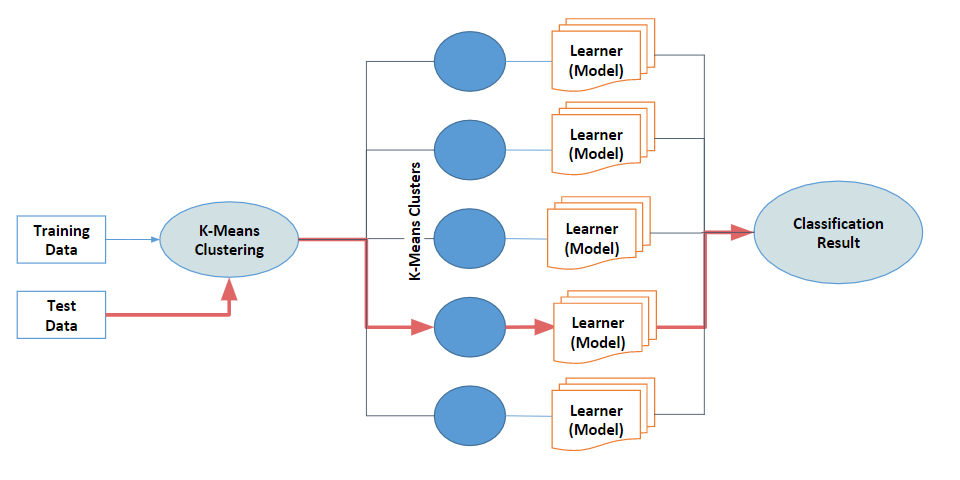
\includegraphics[width=0.8\textwidth]{fig/Models.png}}
        \caption{Model Architecture}
        \label{fig:our_model}
    \end{figure*}
    
    
    
    \subsection{Performance Criteria}
    \label{sssec:performance_criteria}
    For evaluating the described model, this study collects and present the same metrics for performance evaluation as Xu and Fu, in order to compare results. These metrics are precision, recall and f1-score. This multiclass classification problem have 4 classes denoted as Duplicate(C1), Direct Link(C2), Indirect Link(C3) and Isolated(C4). In the results, we present class-wise metrics as well as the average for the whole model.
    
    \begin{table}[h!]
        \centering
        \small
        \resizebox{0.5\linewidth}{!}{\begin{tabular}{@{}cc|c|c|c|c|l@{}}
            \cline{3-6}
            & & \multicolumn{4}{ c| }{Classified as} \\ \cline{3-6}
            & & $C_1$ & $C_2$ & $C_3$ & $C_4$ \\ \cline{1-6}
            \multicolumn{1}{ |c  }{{\rotatebox[origin=c]{90}{Actual}}} &
            \multicolumn{1}{ |c| }{$C_1$} & \cellcolor{lightgray}$C_{11}$ & $C_{12}$  & $C_{13}$ & $C_{14}$  & \\ \cline{2-6}
            \multicolumn{1}{ |c  }{}                        &
            \multicolumn{1}{ |c| }{$C_2$} & $C_{21}$ & \cellcolor{lightgray}$C_{22}$ & $C_{23}$ & $C_{24}$ &  \\ \cline{2-6}
            \multicolumn{1}{ |c  }{}                        &
            \multicolumn{1}{ |c| }{$C_3$} & $C_{31}$ & $C_{32}$ & \cellcolor{lightgray}$C_{33}$ & $C_{34}$ & \\ \cline{2-6}
            \multicolumn{1}{ |c  }{}                        &
            \multicolumn{1}{ |c| }{$C_4$} & $C_{41}$ & $C_{42}$ & $C_{43}$ & \cellcolor{lightgray}$C_{44}$ & \\ \cline{1-6}
        \end{tabular}}
        \caption{Confusion Matrix}
        \label{tab:confusion_matrix}
    \end{table}
    
    Now from the confusion matrix describe above in Table~\ref{tab:confusion_matrix}, it can be observed that the correct predictions are the one with label {\em Cii} for a class {\em Ci}. Now from this we will be able to calculate our evaluation matrixs. So here if a class {\em Ci} has been classified as {\em Cj} then it will be calculated as a wrong classification according to our confusion matrix.
    
    So from the confusion matrix calculation of the precision, recall and F-Score can be done as follows
    
    \begin{equation}
        precision = \frac{C_i_i}{\sum\limits_{i}C_i_j}
    \end{equation}
        \begin{equation}
        recall = \frac{C_i_i}{\sum\limits_{i}C_j_i}
    \end{equation}
        \begin{equation}
        F-Score = \frac{2*recall*precision}{(precision + recall)}
    \end{equation}

    \subsection{Statistical Analysis}
    \label{sssec:Statistical Analysis}
    In order to compare results of the local models with other models, there are two useful tests: significance tests ~\cite{bentler1980significance} and effect size tests ~\cite{rosenthal1994parametric}~\cite{chen2002correlation}. Whereas significance tests tell statistically whether results are distinct enough to be considered different, effect size tells us whether that difference is actually interesting. In order to determine whether the difference in performance of different methods is significant, this study uses the Scott-Knott test, which ranks treatments using a recursive bi-clustering algorithm. At each level, treatments are split where expected value of the treatments has most changed from before. Results in each rank are considered the same according to both significance and effect size tests. Specifically, the Scott-Knott test uses the nonparametric bootstrap ~\cite{efron1982jackknife} method and A12 test.
    

\section{Results}
\label{sect:Result}
    In this section we try to answer the research questions that we have asked as per this experiment. This includes all the experimental results along with our take on that. 
    
    So as part of the experiment this study tries to compare the result of Fu\textquotesingle s DE SVM with our clustered with DE SVM  and clusterer then DE KNN. And also tries to compared the result with XU\textquotesingle s CNN with models from this study. 
    
    \textbf{RQ1}:  {\em Can we reproduce Fu\textquotesingle s results for tuning SVM with differential evolution (DE)?}
    
    This study uses same differential evolution with SVM for both global and local models. Thus to compare with FU's DE with SVM as global model, the first task as part of this experiment was to recreate Fu\textquotesingle s work so that we have a baseline to measure against. The study uses the same SVM from Scikit-learn with the parameters tuned as mentioned in Table~\ref{tab:DE_Parameters}.Here the training time of the DE+SVM model is also compared with Fu\textquotesingle s model. Table~\ref{tab:performance Measure comp} below shows the class by class comparison for all the performance measure this study is using.
    
    From Table~\ref{tab:performance Measure comp} and Figure~\ref{fig:delta_comp_Fu's_ours} it is safe to say that the model this study uses, SVM with DE for hyperparameter tuning ~\cite{duan2003evaluation}~\cite{fu2017easy} is similar to what Fu has used in his paper. It can be observed from this figure that for most of the cases apart from class 3, the model has performed a little better, but the delta between the performance is very small to consider. So to answer RQ1, this study has successfully implemented Fu\textquotesingle s SVM and seeing the results it can be assumed that we will be able to use this implementation to compare this study's results and use this version of DE+SVM implementation~\cite{fu2017easy} for the next part of the experiment.
        \begin{table}
        \centering
        \begin{tabular}{c|p{2cm}|p{2cm}|p{2cm}}
            \rowcolor{darkgray} \textcolor{white}{\textbf{Class}} & \textcolor{white}{\textbf{Precision Avg}} & \textcolor{white}{\textbf{Recall Avg}} & \textcolor{white}{\textbf{F-Score Avg}} \\
            C1 & \begin{tabular}{c|c}
                0.91  & 0.88 \\
             \end{tabular} & \begin{tabular}{c|c}
                0.92  & 0.86 \\
             \end{tabular}  & \begin{tabular}{c|c}
                0.92  & 0.88 \\
             \end{tabular}\\
            \rowcolor{lightgray} C2 & \begin{tabular}{c|c}
                0.92  & 0.85 \\
             \end{tabular} & \begin{tabular}{c|c}
                0.91  & 0.83 \\
             \end{tabular}  & \begin{tabular}{c|c}
                0.91  & 0.84 \\
             \end{tabular}\\
            C3 & \begin{tabular}{c|c}
                0.97  & 0.99 \\
             \end{tabular} & \begin{tabular}{c|c}
                0.99  & 0.99 \\
             \end{tabular}  & \begin{tabular}{c|c}
                0.98  & 0.97 \\
             \end{tabular}\\
            \rowcolor{lightgray} C4 & \begin{tabular}{c|c}
                0.94  & 0.90 \\
             \end{tabular} & \begin{tabular}{c|c}
                0.92  & 0.90 \\
             \end{tabular}  & \begin{tabular}{c|c}
                0.93  & 0.91 \\
             \end{tabular}\\
            Overall & \begin{tabular}{c|c}
                0.94  & 0.91 \\
             \end{tabular} & \begin{tabular}{c|c}
                0.94  & 0.90 \\
             \end{tabular}  & \begin{tabular}{c|c}
                0.93  & 0.90 \\
             \end{tabular}\\
        \end{tabular}
        \caption{Comparison of all performance measure between Our DE\_SVM and Fu\textquotesingle s DE\_SVM }
        \label{tab:performance Measure comp}
    \end{table}
    
    \begin{figure}
        \centering
        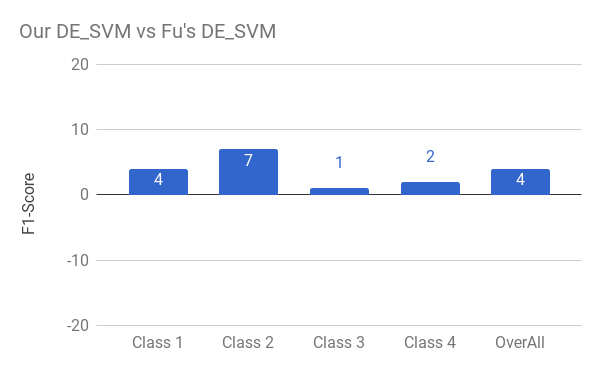
\includegraphics[width=\linewidth]{fig/delta_chart_our_SVM_DE_vs_FU's_SVM_DE.png}
        \caption{Score Delta between our DE\_SVM with Fu\textquotesingle s DE\_SVM. Positive values indicate when our SVM performs better than Fu\textquotesingle s.}
        \label{fig:delta_comp_Fu's_ours}
    \end{figure}
    
    \textbf{RQ2}: {\em  How do the local models compare with global models in both tuned and untuned versions in terms model training time?}
    
    For this part of the experiment, we evaluated the method. As discussed above, this study have used Gap statistic~\cite{mohajer2011comparison}~\cite{tibshirani2001estimating} for finding the best number of clusters, using minimum and maximum number of clusters as 3 and 15, respectively. As part of the experiment 13 clusters are getting best results as per the Gap statistics for the training dataset. 
    
    Now for the next part of the experiment a classifier need to be created on each of the clusters. For this SVM, KNN and both of the algorithms with DE-tuned parameter has been used and implemented. For the normal SVM and KNN the experiment uses the default parameters, described in Table 2. For performing the DE on the learners, the parameters defined in Table 2. 
    
    This study measures the time taken for this model to train which includes time taken by GAP statistic, K-Means training time, and SVM/KNN with DE training time.
    
    We are comparing the results with Fu\textquotesingle s SVM, and XU\textquotesingle s CNN with our models. From the Figure~\ref{fig:time} it can be seen when we cluster data and then create local models on each cluster the study shows good performance improvement. In the case of K-Means then DE with SVM 14 times improvement from using SVM with DE cna be observed. And almost 965x improvement in training time from XU\textquotesingle s CNN. With K-Means then DE with KNN, around 11 times performance improvement can be seen and from XU\textquotesingle s CNN the improvement is around 700 times. Seeing these results we can answer our 2nd question that local models do in fact reduce the runtime by many folds.
    
    \begin{figure}
        \centering
        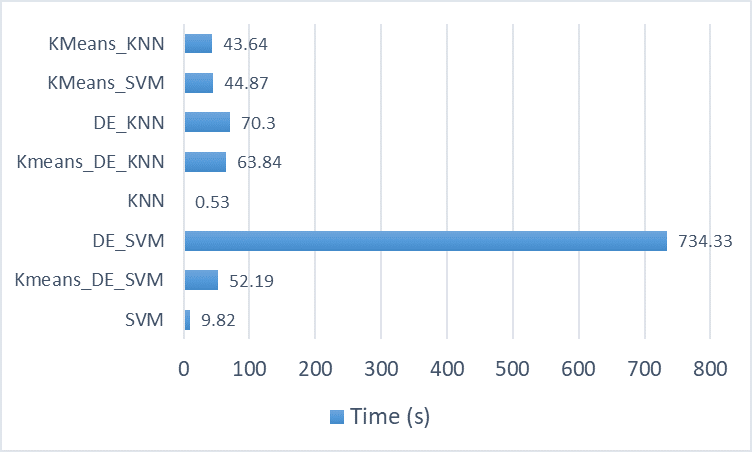
\includegraphics[width=\linewidth]{fig/Time.png}
        \caption{Training time comparison between models (except XU's CNN runtime of 50,400 sec)}
        \label{fig:time}
    \end{figure}
    
    \textbf{RQ3}: {\em  How does the performance of local models compare with global models and state-of-the-art Deep Learner when used with SVM and KNN?} 
    
    \begin{figure}
        \centering
        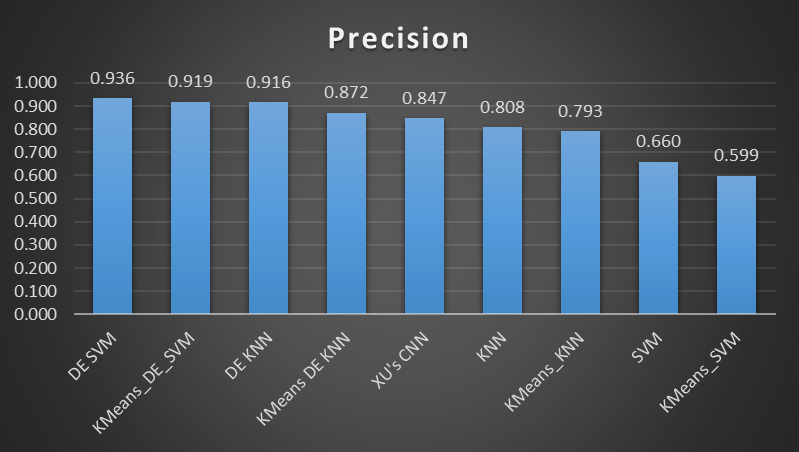
\includegraphics[width=\linewidth]{fig/precision.png}
        \caption{Precision score for all learners}
        \label{fig:precison}
    \end{figure}
    
    The final part of our research question was to check if the local models performance is comparable to Fu's DE\_SVM and the XU's state of the art CNN. To evaluate the performance of the models this study compares performance measures described in Section~\ref{sssec:performance_criteria}. As mentioned in the section, a 10 fold - 10 repeat cross validation has been performed, so all the results are average of 100 models created. 
    
    The 1st performance measure is precision is in Figure~\ref{fig:precison}. The precision of 9 learners discussed in Table~\ref{tab:learners}, for overall class performance is shown in the figure. Now By evaluating the table it can be seen that DE\_SVM's precsion is at 0.94 followed by KMeans\_DE\_SVM at 0.92. Similarly DE\_KNN is followed by KMeans\_DE\_KNN. Both the local models performance almost similar to the global models. But both the models out-performs XU's CNN. Similar trend is also noticeable between without DE versions of the algorithms with default parameters.
    
     \begin{figure}
        \centering
        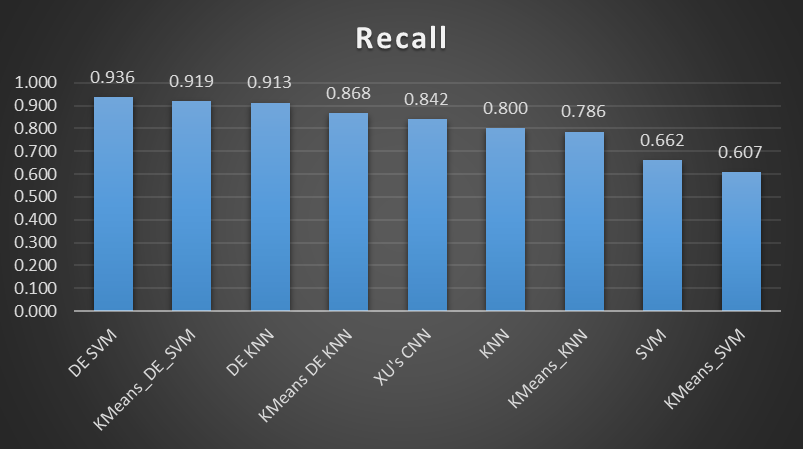
\includegraphics[width=\linewidth]{fig/recall.png}
        \caption{Recall score for all learners}
        \label{fig:Recall}
    \end{figure}
    
    In Figure~\ref{fig:Recall} the performance measures of all the models can be seen in similar way for recall. In here as well the results are similar as precision, global and local models with parameter tuning performs almost similar, but out-performs CNN.
    
    \begin{figure}
        \centering
        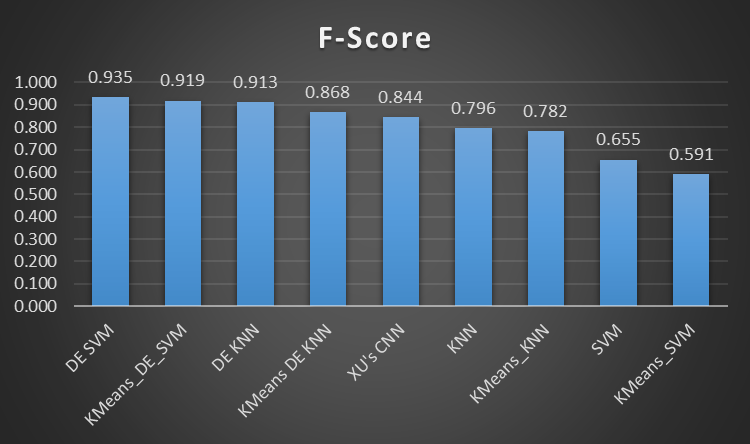
\includegraphics[width=\linewidth]{fig/f-score.png}
        \caption{F1-Score comparison for all learners}
        \label{fig:F1-Score}
    \end{figure}
    
    Figure~\ref{fig:F1-Score} for F-Score measure which is a better understanding of the trade off between precision and recall. Here as well similar results can be observed.
    
    Seeing these results it is assumable that from overall performance evaluation local models performance is almost similar to it's global version. But this study also makes delta comparison between class performance of all the performance criteria for local vs global models for SVM and KNN, and also XU's CNN vs local models. Figure~\ref{fig:Global_vs_Local_DE_SVM} shows the class wise score delta between local KMeans\_DE\_SVM vs global DE\_SVM. We see from the Figure~\ref{fig:Global_vs_Local_DE_SVM} that for all performance criteria and all the classes, the global model performs a slightly better, but the delta is very low.
    
    Figure~\ref{fig:CNN_vs_KMeans_DE_SVM} shows the score delta between XU's CNN and local KMeans\_DE\_SVM. We see in the result that except class 2 recall our models performs better and the delta score is high in class 3 and 4.

    \begin{figure}
        \centering
        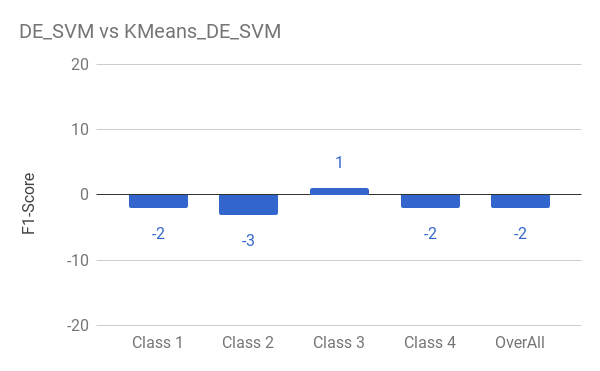
\includegraphics[width=\linewidth]{fig/de_vs_KMenas.png}
        \caption{Class wise Score Delta between Global DE\_SVM vs Local KMeans\_DE\_SVM}
        \label{fig:Global_vs_Local_DE_SVM}
    \end{figure}
    
    \begin{figure}
        \centering
        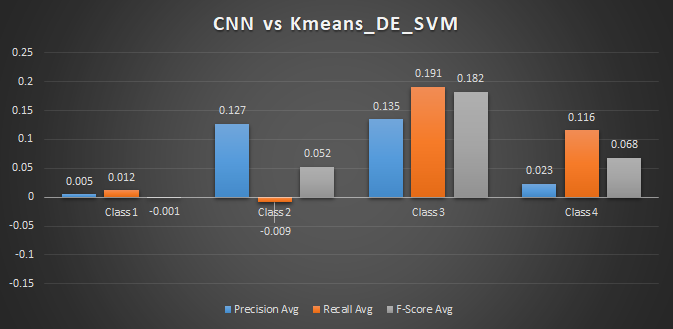
\includegraphics[width=\linewidth]{fig/cnn_vs_Kmeans.png}
        \caption{Class wise score delta between XU's CNN and Local KMeans\_DE\_SVM}
        \label{fig:CNN_vs_KMeans_DE_SVM}
    \end{figure}
    
    Next in Figure~\ref{fig:Global_vs_Local_DE_KNN} class wise score delta of performance matrices between local KMeans\_DE\_KNN vs global DE\_KNN has been recorded, and s similar result vsn be seen, as of the global and local SVM version. in most of the cases the global model's performance is slightly better than local model. In case of XU's CNN vs local KMeans\_DE\_KNN model we see that for class 3 the performance increase is very noticeable for rest of the classes and performance measure the results are almost similar, which can be noticed in Figure~\ref{fig:CNN_vs_KMeans_DE_KNN}.
    
    \begin{figure}
        \centering
        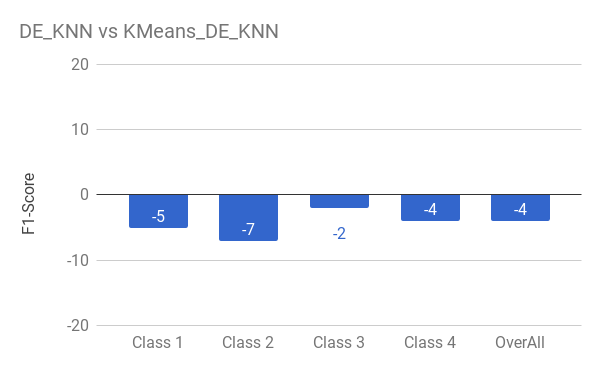
\includegraphics[width=\linewidth]{fig/KNN_vs_KMeans.png}
        \caption{Class wise score delta between Global DE\_KNN vs Local KMeans\_DE\_KNN}
        \label{fig:Global_vs_Local_DE_KNN}
    \end{figure}
    
    \begin{figure}
        \centering
        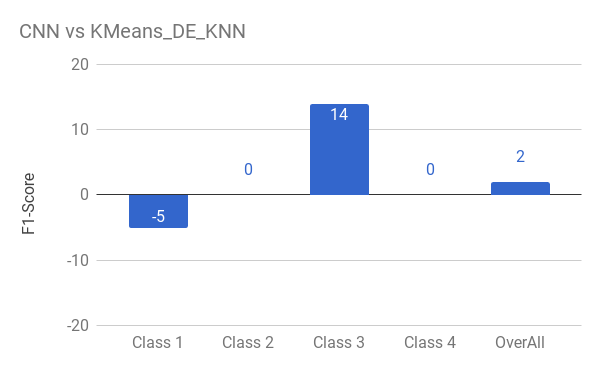
\includegraphics[width=\linewidth]{fig/cnn_vs_Kmeans_Knn.png}
        \caption{Class wise score delta between XU's CNN and Local KMeans\_DE\_KNN}
        \label{fig:CNN_vs_KMeans_DE_KNN}
    \end{figure}
    
    Seeing all the results it can be observed that there is a little difference between the global vs local models as well a difference between state of the art CNN and local models. But observing the score delta charts we see the difference is very small most of the time. This study analysis if these performance measure difference is statistically significant or not. So we ranked the models using scott-knott test as mentioned in Section~\ref{sssec:Statistical Analysis}. The test was conducted on all the performance measures separately with all the results from 10 fold - 10 repeat validations.
    
    \begin{table}[h!]
        \centering
        {\small   \begin{tabular}{l@{~~~~}l@{~~~~}r@{~~~~}r@{~~}c@{}r}
        \multicolumn{1}{l}{\textbf{Rank}}& \textbf{Model} & \textbf{med.} & \textbf{IQR} & \\ 
         \rowcolor{lightgray}\arrayrulecolor{lightgray}
        \textbf{Precision} & \textbf{} & \textbf{} & \textbf{} & \\\hline
          1 &        KMeans\_SVM &    58  &  2 & \quart{57}{1}{60}{2} \\ \hline
          2 &         SVM &    66  &  0  & \quart{66}{0}{66}{0} \\ \hline
          3 &        KMeans\_KNN  &    78  &  0  & \quart{78}{0}{78}{0} \\ \hline
          4 &       KNN &    81   &  0 & \quart{81}{0}{81}{0} \\ \hline
          5 &        CNN &    85  &  0 & \quart{85}{0}{85}{0} \\   
          5 &         KMeans\_DE\_KNN &    87   &  3 & \quart{84}{2}{88}{2} \\\hline
          6 &        KMeans\_DE\_SVM &    92 &  2 & \quart{91}{0}{93}{2} \\
          6 &        DE\_KNN &    93  &  1 & \quart{83}{10}{93}{0} \\\hline
          7 &       DE\_SVM &    94  &  1  & \quart{91}{2}{94}{1} \\\hline 
    
        \end{tabular}} 
    \caption{Scott-Knott ranking for Precision}
    \label{tab: Scott-Knott ranking for Precision}
    \end{table}
    
    \begin{table}[h!]
        \centering
        {\small   \begin{tabular}{l@{~~~~}l@{~~~~}r@{~~~~}r@{~~}c@{}r}
        \multicolumn{1}{l}{\textbf{Rank}}& \textbf{Model} & \textbf{med.} & \textbf{IQR} & \\ 
         \rowcolor{lightgray}\arrayrulecolor{lightgray}
        \textbf{Recall} & \textbf{} & \textbf{} & \textbf{} & \\\hline
          1 &        KMeans\_SVM &    59  &  2 & \quart{58}{1}{60}{2} \\ \hline
          2 &         SVM &    66  &  0  & \quart{66}{0}{67}{1} \\
          3 &        KMeans\_KNN  &    79  &  1  & \quart{79}{0}{80}{1} \\ \hline
          3 &       KNN &    80   &  0 & \quart{80}{0}{80}{0} \\ \hline
          4 &        CNN &    84  &  0 & \quart{84}{0}{84}{0} \\   
          4 &         KMeans\_DE\_KNN &    87   &  3 & \quart{84}{1}{88}{3} \\\hline
          5 &        KMeans\_DE\_SVM &    92 &  2 & \quart{91}{0}{93}{2} \\
          5 &        DE\_KNN &    93  &  1 & \quart{83}{10}{93}{0} \\
          5 &       DE\_SVM &    94  &  1  & \quart{92}{1}{94}{1} \\\hline 
    
        \end{tabular}} 
    \caption{Scott-Knott ranking for Recall}
    \label{tab: Scott-Knott ranking for Recall}
    \end{table}
    
    \begin{table}[h!]
        \centering
        {\small   \begin{tabular}{l@{~~~~}l@{~~~~}r@{~~~~}r@{~~}c@{}r}
        \multicolumn{1}{l}{\textbf{Rank}}& \textbf{Model} & \textbf{med.} & \textbf{IQR} & \\ 
        \rowcolor{lightgray}\arrayrulecolor{lightgray}
        \textbf{F-Score} & \textbf{} & \textbf{} & \textbf{} & \\\hline
          1 &        KMeans\_SVM &    60  &  1 & \quart{59}{0}{61}{2} \\ \hline
          2 &         SVM &    65  &  1  & \quart{65}{0}{66}{1} \\
          3 &        KMeans\_KNN  &    79  &  1  & \quart{78}{1}{79}{0} \\ \hline
          3 &       KNN &    80   &  0 & \quart{79}{1}{80}{0} \\ \hline
          4 &        CNN &    84  &  0 & \quart{84}{0}{84}{0} \\   
          4 &         KMeans\_DE\_KNN &    87   &  3 & \quart{84}{1}{88}{3} \\\hline
          5 &        KMeans\_DE\_SVM &    92 &  2 & \quart{91}{0}{93}{2} \\\hline
          6 &        DE\_KNN &    93  &  0 & \quart{83}{10}{93}{0} \\
          6 &       DE\_SVM &    94  &  1  & \quart{91}{2}{94}{1} \\\hline 
    
        \end{tabular}} 
    \caption{Scott-Knott ranking for F-Score}
    \label{tab: Scott-Knott ranking for F-Score}
    \end{table}
    

    From the results of the Scott-Knott test it can be seen that in case of precision in Table~\ref{tab: Scott-Knott ranking for Precision} the DE\_SVM and KMeans\_DE\_SVM have separate ranking as 6 for  KMeans\_DE\_SVM and 7 for DE\_SVM and as well XU's CNN is at rank 5. So in case of precision it can be observed that the results of these 3 models are statistically different, but looking at the median it can be said that, although they are different they have very similar or we can say comparable results. It can be seen in Table~\ref{tab: Scott-Knott ranking for Recall} DE\_SVM and KMeans\_DE\_SVM are ranked similar, so in case of recall their performance is statistically same, both ranked at 5, while XU's CNN is ranked at 4. And the results are similar in case of F-Score as seen in Table~\ref{tab: Scott-Knott ranking for F-Score}, with DE\_SVM ranked at 6 and KMeans\_DE\_SVM ranked at 5 and XU's CNN ranked at 4.
    
    So seeing all the results of difference perfromance measures and ranking test that although local models have a slightly lower measure than global models in case of precision and f-score and a slightly better performance in recall, overall the local models performs almost similar to their global part and the models performance is comparable to state of the art convolution neural networks.
    
    
\section{THREATS TO VALIDITY}
\label{sect:THREATS TO VALIDITY}
    Threats to internal validity of our work includes the fact that this study started the experiment directly based on the code repository that was provided in the "Easy Over Hard" paper. Since we forked Fu's GitHub Repo link and collected the metrics for DE\_SVM that the result's validity are directly linked to the validity of his results. In order to continue with the other learners described in Table~\ref{tab:learners}, we added additional code and scripts to the code base . 
    
    Most of the Deep Learning methods or tools from papers in SE are not publicly available or they are too complicated to implement, the XU's CNN is also not publicly available. Along with that CNNs normally have multiple layers and thousands or weights and connections between layers, a very small deviation from original network can results in huge difference in performance. So this paper does not implement XU's CNN network, all of XU's result data is publicly available along with the hardware configuration(2.5GHz,16GB ram on 64bit platform), this experiment uses almost similar hardware configuration with 3.00GHz processor with 16GB ram, running on 64bit platform and this paper implemented FU's DE\_SVM in our machine configuration and got runtime that is quite similar. So it can assumed that this experiment's runtimes will be comparable with FU's and XU's models.
    
    Also In the "Easy Over Hard" paper, Fu also points out that since the original Word Embedding + SVM baseline method was not available publicly, he implemented his own version and got results very similar to the ones reported on Xu's study. As this study directly uses the Word Embedding model created by Fu, the results validity depends on Fu's implementation of the Word Embedding model.
    
    In this paper, the performance metrics that  are reported for the experiments - recall, precision, f1-score, and accuracy - are the same ones reported on Fu's DE\_SVM paper and the XU's CNN  paper. The experimental results for the learner combination in Table A are very much comparable to the DE\_SVM results. The reason this study tries building local models using cluster-first approach was to capture any local similarities or properties that the data domain might have. It worked out well in this experimen, but that does not mean that other external text mining datasets will have any local patterns that can be captured. It might be the case there are not any locally specific characteristics and hence global models with tuned standard learners might produce similar results as local models. But it is very much possible that there might be local nuances in the dataset that can be well captured by the clusters and hence the models trained on the subsets might be better at prediction.


\section{CONCLUSION}
\label{sect:CONCLUSION}
    In this paper we try to investigate significance of local models from the perspective of significant reduction in training time with comparable performance then global models and Deep Learning system for predicting knowledge unit's relatedness on Stack Overflow. This study shows procedure to cluster the data first and then build local models on each cluster separately, then use the clustering algorithms with the local classification algorithm together to predict. Algorithm's run time depends upon the size of the input, each local model reduces the training time by having to run on a subset of data and thus reducing the overall run time. This experimental result shows -
    
    \begin{itemize}
        \item Clustering the data first and then building local models on those subsets of data shows significant reduction in runtime.
        \item Using KMeans on the Word Embedding model first to cluster the data into smaller subsets and then running SVM and KNN with their DE versions showed runtime reduction as large as 965 times for KMeans\_DE\_SVM version with CNN and almost 14 times improvement than its global DE\_SVM version.
        \item The performance in term of precision, recall and F-score is almost similar to its global counter part and sometime better then the XU's CNN model.
    \end{itemize}
    
    With this paper we also like to propagate the importance of "No Free Lunch Theorem" ~\cite{wolpert1997no} in machine learning. This experiment discovered each local learner with DE is fine tuned with separate set of parameter values. That proves the clustered data are different from one another and thus building local models creates more specificity in prediction. 
    
    
    For future work, we suggest trying several variations of this experiment - 
    
    \begin{itemize}
        \item In this experiment we tune the local models separately, tuning all the local models along with the clustering algorithm together might produce some interesting results.
        \item Trying to find correlation between number of cluster and training time and performance might give us effect of number of clusters on the prediction model.
    \end{itemize}
    

\bibliographystyle{ACM-Reference-Format}
\bibliography{700faster} 

\end{document}